\documentclass[12pt]{article}
\usepackage[catalan]{babel}
\usepackage[utf8]{inputenc}
\usepackage{listings}
\usepackage{color}
\usepackage{graphicx}
\usepackage{verbatim}
\usepackage[obeyspaces]{url}
\usepackage{appendix}
\usepackage{dirtytalk}

\definecolor{codegreen}{rgb}{0,0.6,0}
\definecolor{codegray}{rgb}{0.5,0.5,0.5}
\definecolor{codepurple}{rgb}{0.58,0,0.82}
\definecolor{backcolour}{rgb}{0.95,0.95,0.92}
 
\lstset{
	backgroundcolor=\color{backcolour},   
	breaklines=true, 
	numbers=left,
	basicstyle=\footnotesize,
	backgroundcolor=\color{backcolour},   
    commentstyle=\color{codegreen},
    keywordstyle=\color{magenta},
    numberstyle=\tiny\color{codegray},
    stringstyle=\color{codepurple},
    basicstyle=\footnotesize,
    breakatwhitespace=false,         
    breaklines=true,                 
    captionpos=b,                    
    keepspaces=true,                 
    numbers=left,                    
    numbersep=5pt,                  
    showspaces=false,                
    showstringspaces=false,
    showtabs=false,                  
    tabsize=2
}
\setlength{\parindent}{0pt}

\begin{document}
\begin{titlepage}
		\centering
		
\includegraphics[width=0.5\textwidth]{imatges/logo.png}\par\vspace{1cm}
		{\huge\bfseries Projecte final\par}
		\vspace{1cm}
		{\scshape\Large Màster en enginyeria informàtica\par}
		\vspace{1.5cm}
		{\Large\itshape Oscar Galera i Alfaro\par}
		\vspace{1cm}
		{\Large\itshape Mineria de dades\par}
		\vspace{2cm}
		\vfill
		\vfill
		{\large \today\par}
\end{titlepage}
\clearpage
\tableofcontents
\clearpage
\listoffigures


\clearpage
%%%%%%%%%%%%%%%%%%%%%%XARXA NEURONAL%%%%%%%%%%%%%%%%%%%%%%%%
\section{Què és una xarxa neuronal?}
En aquesta secció es descriuran els components més importants que composen una xarxa neuronal.
\begin{figure}[h!]
	\centering
	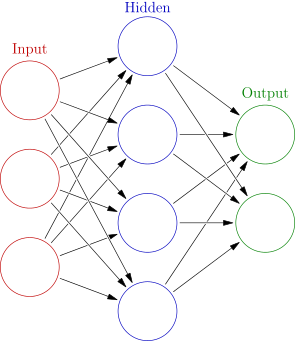
\includegraphics[scale=.5]{imatges/xnn.png}
	\caption{Xarxa neuronal}
\end{figure}
\\\\Una xarxa neuronal, és una estructura de dades dissenyada per a simular (en la mesura del possible) el comportament del cerbell humà. El disseny d'aquesta estructura es fonamenta en diferents capes de neurones interconnectades entre elles i que a través d'un procés iteratiu, són capaces d'ajustar-se i d'aquesta manera adquirir coneixement.
\\\\Una xarxa neuronal sempre tindrà una única capa de neurones d'entrada\footnote{Aquestes neurones d'entrada representen les variables independents sobre les que es vol fer l'anàlisi.}, $n$ capes de neurones internes (depenent del problema que es vol resoldre) i 1 capa de neurones de sortida.
\begin{itemize}
	\item Neurones de la capa d'entrada: emulen sensors que perceben la informació que es vol processar.
	\item Neurones de les capes internes: són les neurones que adquireixen el coneixement.
	\item Neurones de la capa de sortida: són les neurones que proporcionen els resultats obtinguts.
\end{itemize}


%%%%%%%%%%%%%%%%%%%%%%NEURONA%%%%%%%%%%%%%%%%%%%%%%%%
\clearpage
\subsection{Què és una neurona?}
Les neurones són els blocs bàsics en que es recolçen les xarxes neuronals. La seva funcionalitat treballant de forma individual no serveix, però si que serveix si es treballa de forma estrcturada amb grans quantitas d'aquestes.
\begin{figure}[h!]
	\centering
	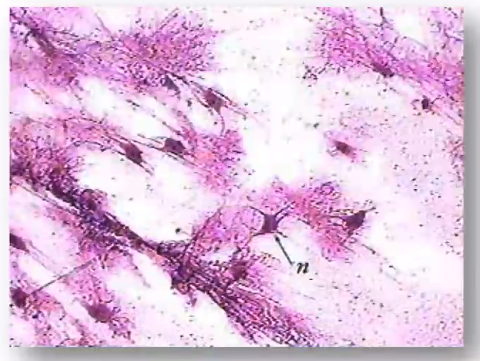
\includegraphics[scale=0.4]{imatges/neurona/1real.png}
	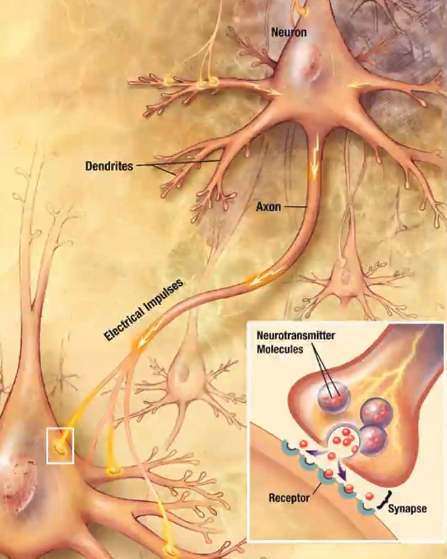
\includegraphics[scale=0.4]{imatges/neurona/3estructura.png}
	\caption{Anatomia d'una neurona real.}
\end{figure}
\\\\Una neurona es composa principalment de:
\begin{itemize}
	\item Núcli.
	\item Dendrites (emissor).
	\item Axó (receptor).
\end{itemize}
La interconexió de les neurones, es fa a través de l'enviament i recepció de impulsos elèctrics (\textit{synapses}).
\pagebreak
\clearpage
\begin{figure}[h!]
	\centering
	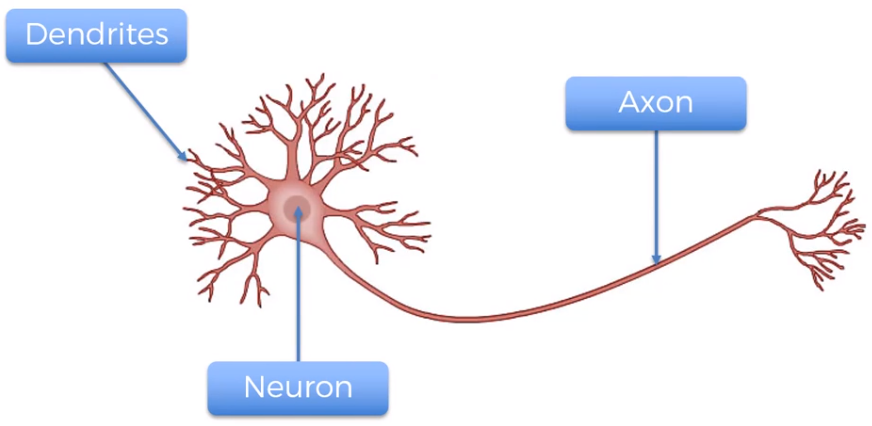
\includegraphics[scale=0.4]{imatges/neurona/9parts.png}
	\caption{Parts d'una neurona.}
\end{figure}
Una xarxa neuronal es pot representar a través d'una caixa negre on hi ha un conjunt d'entrades (neurones d'entrada) i una o varies sortides (neurones de sortida).
\begin{figure}[h!]
	\centering
	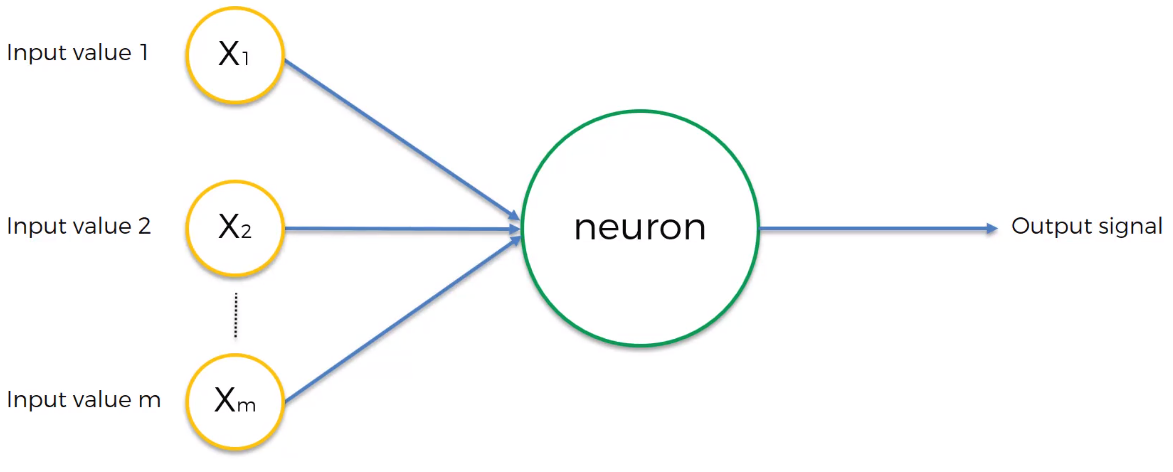
\includegraphics[scale=0.2]{imatges/neurona/5estructura.png}
	\caption{Xarxa neuronal simple.}
\end{figure}
\\\\Les neurones tenen la capacitat d'aprendre, això s'aconsegueix gràcies als pessos assignats a les connexions entre neurones (\textit{weights}), que determinen el grau d'importancia que té cada una de les neurones d'entrada. Aquests valors s'actualitzen a través de la tècnica del \textbf{\textit{backpropagation}} (secció \ref{bp}) que utilitza el mètode matemàtic del \textbf{descens del gradient} (secció \ref{dg} i \ref{dge}). 
\\\\El fet d'actualitzar el valor per aquests pesos, determinarà el grau de qualitat de la xarxa neuronal.
\begin{figure}[h!]
	\centering
	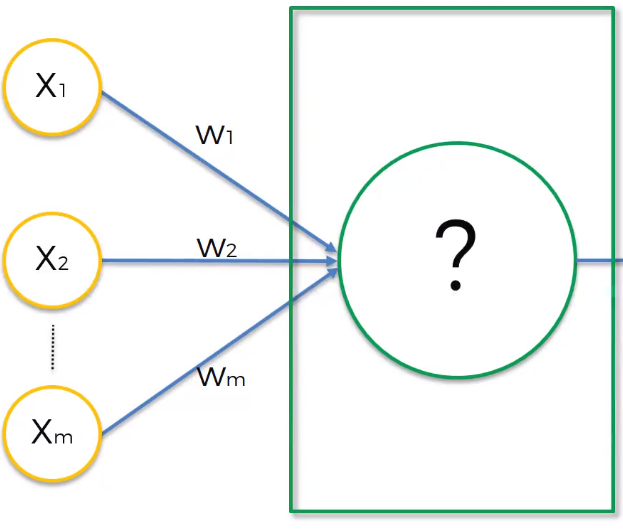
\includegraphics[scale=0.2]{imatges/neurona/6pes.png}
	\caption{Pes (\textit{weights}) de les connexions entre neurones.}
\end{figure}
\pagebreak
\\\\Amb els valors que rep una neurona de la resta de neurones d'entrada, cal generar un valor que serà la sortida, per això cal fer una agregació de valors a través de la \textbf{funció d'activació} (secció \ref{fa}).
\begin{figure}[h!]
	\centering
	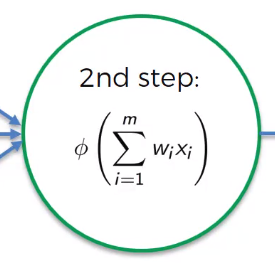
\includegraphics[scale=0.4]{imatges/neurona/7activacio.png}
	\caption{Agregació de valors d'entrada.}
\end{figure}
\\\\Descrits els diferents components d'una neurona, la integració d'aquesta dins d'una xarxa de neurones es pot representar a través de la següent imatge.
\begin{figure}[h!]
	\centering
	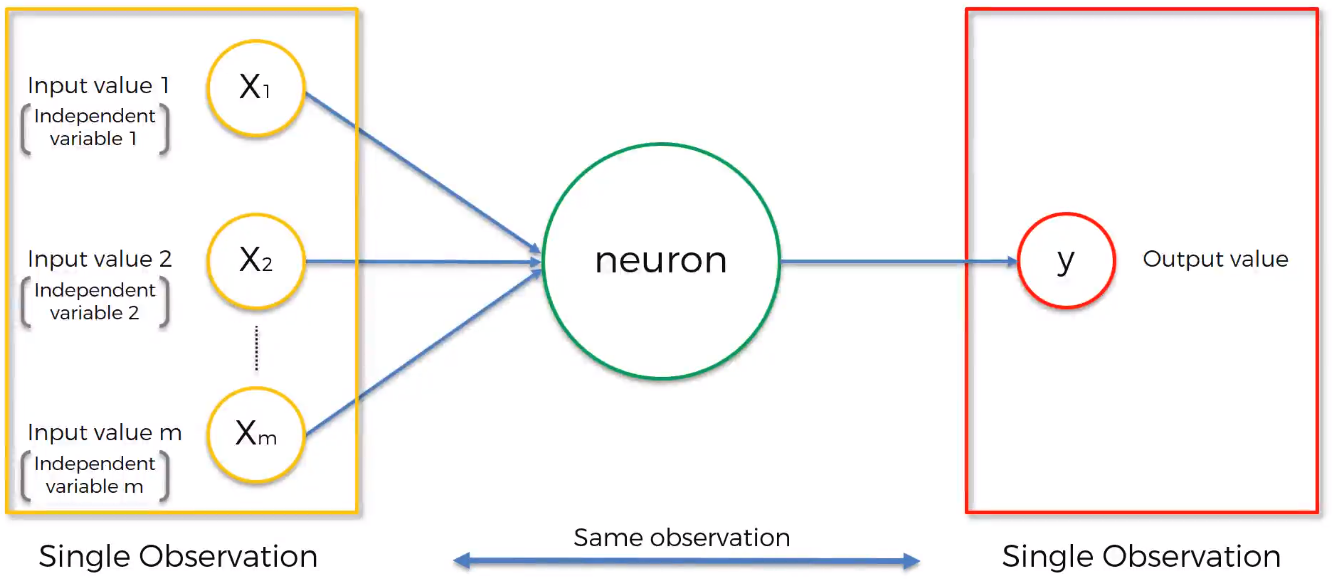
\includegraphics[scale=0.3]{imatges/neurona/8completa.png}
	\caption{Integració d'una neurona en una xarxa neuronal.}
\end{figure}
S'ha de tenir en compte que el procés d'aprenentatge d'una xarxa neuronal és iteratiu, i que tots els valors de les neurones d'entrada corresponen a una mateixa observació i el valor de sortida al resultat d'aquesta observació.



\clearpage
%%%%%%%%%%%%%%%%%%%%%%FUNCIÓ D'ACTIVACIÓ%%%%%%%%%%%%%%%%%%%%%%%%
\subsection{La funció d'activació \label{fa}}
Les funcions d'activació serveixen per calcular el valor que emetrà una neurona com a sortida. Les funcions d'activació més típics són:
\begin{itemize}
	\item Threshold function.
	\item Sigmoid.
	\item Rectifier function.
	\item Hyperbolic tangent (tanh).
\end{itemize}
\subsubsection{Threshold function}
El rang de possibles valors per aquesta funció és 0 o 1, això fa que sigui una funció molt rigida i que s'adapti perfectament a casos on volem una sortida binaria.
\begin{figure}[h!]
	\centering
	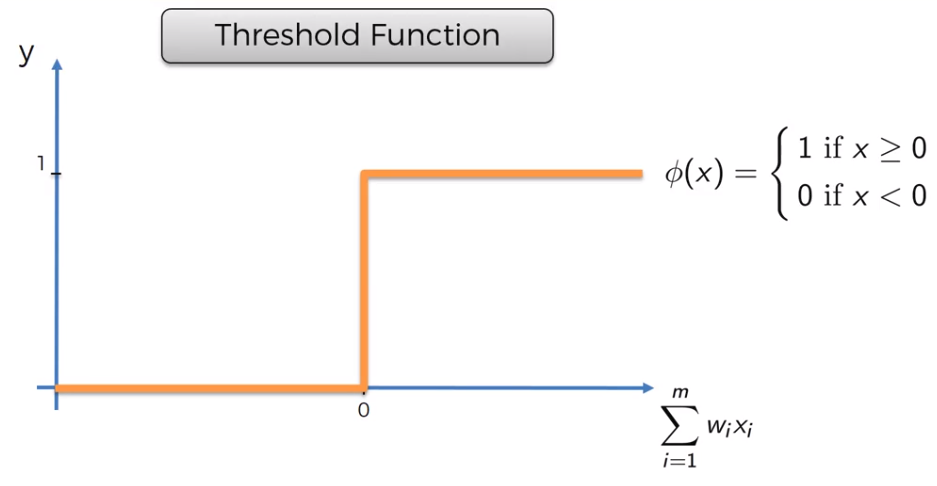
\includegraphics[scale=0.3]{imatges/fa/1threshold.png}
	\caption{Threshold function.}
\end{figure}

\subsubsection{Sigmoid}
El rang de valors per aquesta funció va de (0, 1) i es sol utilitzar molt com a funció d'activació en l'última capa de neurones, per calcular probabilitats.
\begin{figure}[h!]
	\centering
	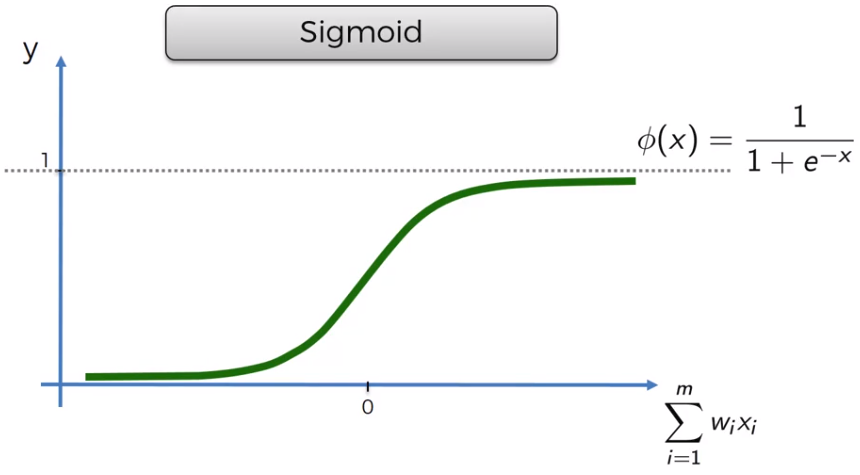
\includegraphics[scale=0.3]{imatges/fa/2sigmoid.png}
	\caption{Sigmoid function.}
\end{figure}
\\\\\\És una funció que s'utilitza molt en la regressió logistica.

\subsubsection{Rectifier function}
El rang d'aquesta funció va de [0, $x$], on $x$ correspon a la suma ponderada dels valors d'entrada de la capa de neurones anterior.
\begin{figure}[h!]
	\centering
	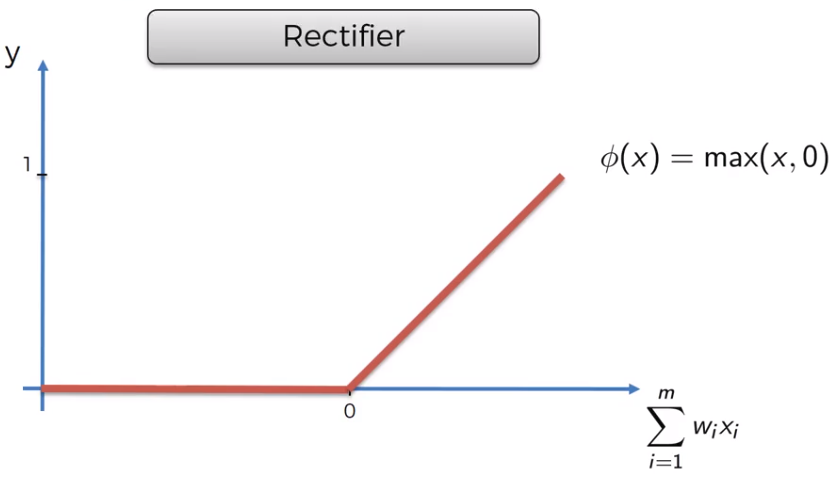
\includegraphics[scale=0.3]{imatges/fa/3rectifier.png}
	\caption{Rectifier function.}
\end{figure}

\subsubsection{Hyperbolic tangent}
El rang d'aquesta funció va de (-1, 1) i és molt similar a la funció sigmoid.
\begin{figure}[h!]
	\centering
	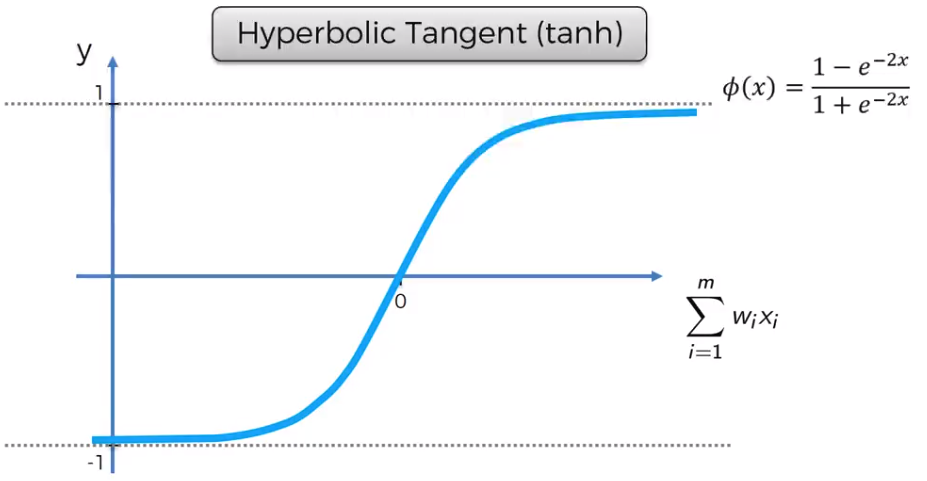
\includegraphics[scale=0.3]{imatges/fa/4tanh.png}
	\caption{Hyperbolic tangent.}
\end{figure}

\subsection{Funcions d'activació sobre una xarxa neuronal}
Per a cada neurona interna, s'ha de definir una funció d'activació, per això es poden seguir diferents tècniques.
\begin{itemize}
	\item Assignar una mateixa funció d'activació a tota la xarxa neuronal (rigida però sencilla de desenvolupar i mantenir).
	\item Assignar una mateixa funció d'activació a nivell de capa de neurones interna.
	\item Assignar una funció d'activació diferent per a cada neurona (complexe però potent).
\end{itemize}
La tècnica a utilitzar dependrà sempre del tipus de problema a resoldre i de la potencia disponible.
\begin{figure}[h!]
	\centering
	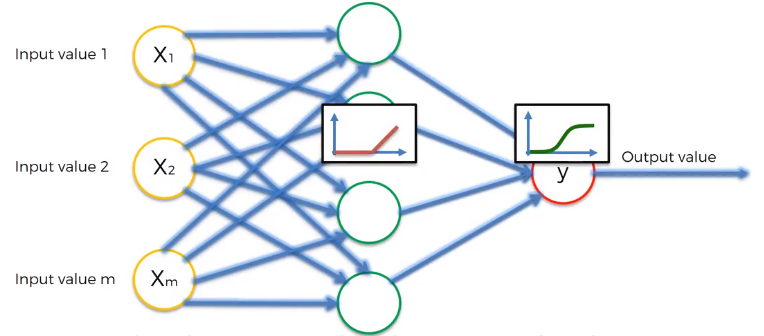
\includegraphics[scale=0.3]{imatges/fa/5complet.png}
	\caption{Aplicació de funcions d'activació sobre una xarxa neuronal.}
\end{figure}



\clearpage
%%%%%%%%%%%%%%%%%%%%%%COM FUNCIONEN?%%%%%%%%%%%%%%%%%%%%%%%%
\subsection{Com funcionen?}
El funcionament de les xarxes neuronals és basa en la configuració que s'ha de fer sobre les capes de neurones internes. Per veure millor com funcionen, s'utilitzarà un exemple de possible aplicació real, en la que es disposa d'un conjunt de paràmetres (dimensions, nombre de lavabos, distància del centre de la ciutat i edat) i es vol especular el preu que pot tenir una vivendra sengons les seves propietats.
\\\\A nivell de neurona, s'ha d'elegir quins paràmetres actuen sobre el el seu càlcul i crear una \textit{synapse} que enllaçi les neurones. 
\\\\En aquests exemple, la primera neurona s'utilitza per influir en l'especulació del preu en base a les mides de la vivenda i la distància que està del centre de la ciutat. 
\\\\De forma intuitiva es pot pensar que les vivendes més grans i que estàn properes al centre de la ciutat són més cares, i per això, la primera neurona interna influirà en el preu en base aquests dos paràmetres.
\begin{figure}[h!]
	\centering
	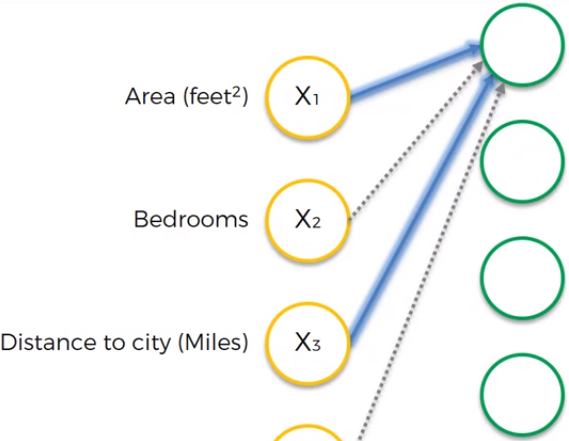
\includegraphics[scale=0.3]{imatges/funcionament/1basic.png}
	\caption{Configuració d'una neurona.}
\end{figure}
\\\\D'aquesta manera, una possible configuració completa d'una xarxa molt sencilla per calcular el preu pot ser com en la següent imatge.
\pagebreak
\clearpage
\begin{figure}[h!]
	\centering
	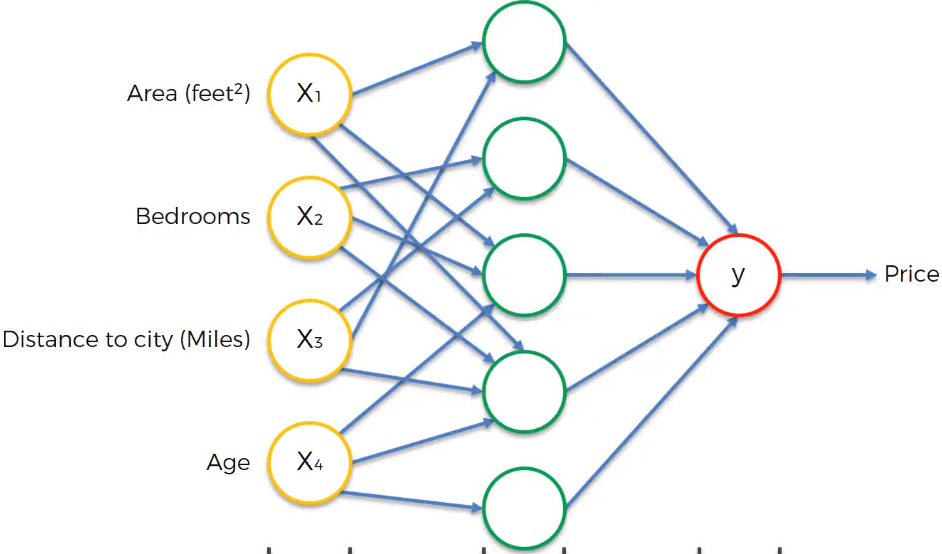
\includegraphics[scale=0.3]{imatges/funcionament/2completa.png}
	\caption{Configuració completa d'una xarxa neuronal sencilla.}
\end{figure}
Les neurones que no tenen inpacte en el calcul no es representen utilitzant syapses, això es pot interpretar com que tenen un impacte nul sobre aquell càlcul.

\clearpage
%%%%%%%%%%%%%%%%%%%%%%COM APRENEN?%%%%%%%%%%%%%%%%%%%%%%%%
\subsection{Com aprenen?}
Com ja s'ha dit anteriorment, les xarxes neuronals es basen en un mecanisme d'aprenentatge iteratiu amb el qual van adquirint coneixement a mesura que guanyen experiència. Per aquest motiu, és necessari dividir les etapes de funcionament d'una xarxa neuronal en:
\begin{itemize}
	\item \textbf{Etapa d'entrenament:} en aquesta etapa es proporcionen multiples exemples a partir dels quals s'adquireix la gran majoria del coneixement. S'ha de tenir en compte que durant aquest procés cal saber el resultat correcte per obtenir una xarxa ben entrenada.
	\item \textbf{Etapa de test:} en aquesta etapa es posa a prova la xarxa, proporcionant noves dades i analitzant els resultats. En cas de comptar amb el resultat correcte per aquestes dades, la xarxa pot continuar aprenent.
\end{itemize}
Durant l'etapa d'entrenament i un cop s'obté el resultat proporcionat de la xarxa, cal comprar-lo amb el resultat real i extreure un valor que representi la distància que hi ha entre el valor preedit i el correcte. Aquesta magnitut s'extreu a partir de la funció de cost. 
\begin{figure}[h!]
	\centering
	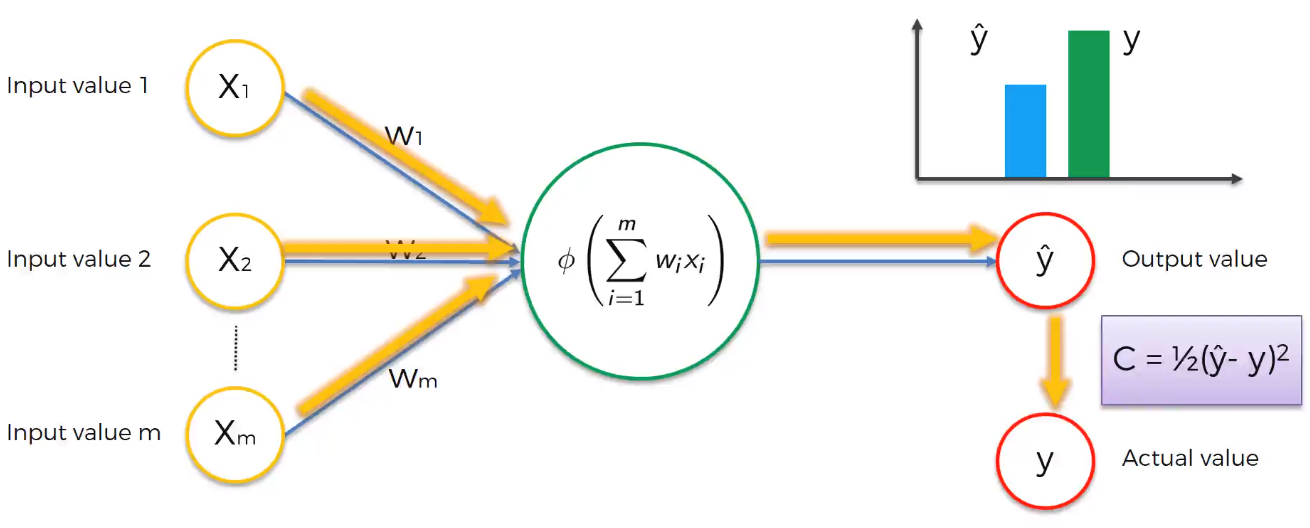
\includegraphics[scale=0.3]{imatges/aprendre/1aprendre.png}
	\caption{Funció de cost.}
\end{figure}
El valor proporcionat per la funció de cost, s'utilitza com entrada del mecanisme d'adaptació d'adaptació de la xarxa(\textit{backpropagation}).
\begin{figure}[h!]
	\centering
	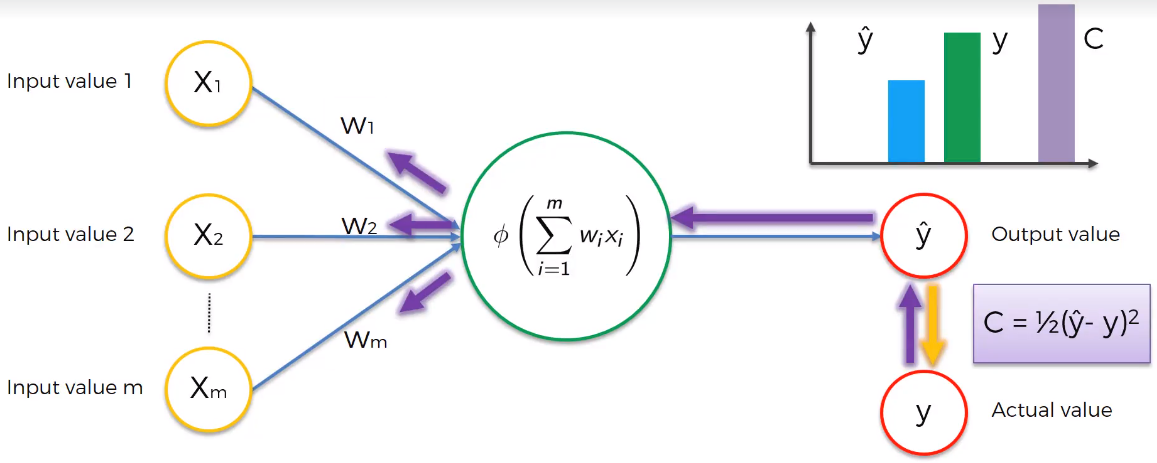
\includegraphics[scale=0.3]{imatges/aprendre/2bp.png}
	\caption{\textit{Backpropagation}.}
\end{figure}
\clearpage
%%%%%%%%%%%%%%%%%%%%%%DESCENS DEL GRADIENT%%%%%%%%%%%%%%%%%%%%%%%%
\subsection{Descens del gradient\label{dg}}


\clearpage
%%%%%%%%%%%%%%%%%%%%%%DESCENS DEL GRADIENT ESTOCÀSTIC%%%%%%%%%%%%%%%%%%%%%%%%
\subsection{Descens del gradient estocàstic\label{dge}}


\clearpage
%%%%%%%%%%%%%%%%%%%%%%BACKPROPAGATION%%%%%%%%%%%%%%%%%%%%%%%%
\subsection{Backpropagation\label{bp}}


\clearpage
\section{Classificació utilitzant una xarxa neuronal}
\subsection{Dades}
\subsection{Problema}
\subsection{Eines a utilitzar}
\subsection{Classificació}
Els passos a seguir per aplicar la classificació utilitzant una xarxa neuronal són.
\begin{enumerate}
	\item Preprocessament de les dades.
	\item Creació de la xarxa neuronal.
	\item Classificació.
	\item Evaluar la precissió del model.
\end{enumerate}
\subsubsection{Processament de les dades}

%%%%%%%%%%%%%%%BIBLIOGRAFIA%%%%%%%%%%%%%%%%%
\clearpage
\begin{thebibliography}{9}
	\bibitem{ANN}\textit{Xarxa neuronal}:
  	\\\path{https://en.wikipedia.org/wiki/Artificial_neural_network}
	\bibitem{AF1}\textit{Deep sparse rectifier neural networks}:
  	\\\path{http://proceedings.mlr.press/v15/glorot11a/glorot11a.pdf}
	\bibitem{FC}\textit{Funcions de cost més tipiques}:
  	\\\path{https://stats.stackexchange.com/questions/154879/a-list-of-cost-functions-used-in-neural-networks-alongside-applications}
\end{thebibliography}

\clearpage
\begin{appendices}
\section{Codi}
\end{appendices}
\end{document}